\section{Cylc Introduction}


\subsection{The suite.rc File}

A cylc suite is a collection of files located within a directory called the
suite directory. The suite is configured by a single suite.rc file.
The suite.rc file uses a nested INI based format where sections are denoted
by square brackets, sub-sections by double square brackets and
sub-sub-sections by triple square brackets.

\begin{lstlisting}[language=suiterc]
[section]
    [[subsection]]
        option = value
\end{lstlisting}

There are five top level sections that can be present in a suite.rc file. The
three main ones are:

\begin{tabular}{ll}
\begin{lstlisting}
[cylc]
\end{lstlisting} & Used for suite-level configuration. \\
\begin{lstlisting}
[scheduling]
\end{lstlisting} & Defines the logic of the suite enabling cylc to determine
when tasks are ready to run. \\
\begin{lstlisting}
[runtime]
\end{lstlisting} & Defines the tasks themselves, what to execute, where and
how. \\
\end{tabular}


\subsection{Hello World in cylc}

The simplest working example of a cylc suite is given below. This suite
contains a single task named \lstinline{hello_world} which waits 5 seconds
then outputs the text ``Hello World!'' to standard out. The task is defined in
in the \lstinline=[runtime]= section and cylc is told to run the task by the
\lstinline{graph = hello_world} part.

\begin{lstlisting}[language=suiterc, title=hello world example]
[scheduling]
    [[dependencies]]
        graph = hello_world
[runtime]
    [[hello_world]]
        script = sleep 5; echo "Hello World!"
\end{lstlisting}

To run a new suite there are three things that must be done:

\begin{enumerate}
    \item The suite must be registered with cylc
    \item (optionally) the suite can be validated to ensure there are no errors
            in the suite.rc file.
    \item Finally, we can run the suite.
\end{enumerate}

To do this we can use the \lstinline[language=bash]{rose suite-run} command.
This command requires a rose-suite.conf file which should sit alongside the
suite.rc. The rose-suite.conf file can be empty.

\begin{lstlisting}[language=bash]
$ touch rose-suite.conf
$ rose suite-run
\end{lstlisting}

For this tutorial we will be using the \lstinline{rose suite-run} command
though these three steps can be undertaken without using rose using the
following cylc commands.

\begin{lstlisting}[language=bash]
$ cylc register hello_world /path/to/suite/
$ cylc validate hello_world
$ cylc run hello_world
\end{lstlisting}

\paragraph*{Demo}
To run the hello world example, create a directory called hello\_world. This
will be our suite directory.

Next copy the ``hello world example'' code into a suite.rc file within that
directory.

Finally run the following commands:

\begin{lstlisting}[language=bash]
$ cd hello_world  # move to the suite directory
$ touch rose-suite.conf  # create an empty rose-suite.conf file
$ rose suite-run  # run the suite
\end{lstlisting}

If successful cylc will generate some output then a window will open. This is
the cylc monitoring and control tool which displays the current status of
your suite. In the cylc gui you should briefly see the task
\lstinline{hello_world}
displayed with a coloured square next to it. The colour of the square
represents the state of the task
(for example green means the task is running and gray that it has succeeded).
Once the hello\_world task has succeeded, having no more tasks to run the suite
will automatically shut down.


\subsection{Tasks}

To convert a script into a cylc task the script should be placed inside a
`bin` directory alongside the suite.rc file in the suite directory.

\begin{lstlisting}[language=]
suite-directory/
|-- bin/
|   `-- get-host-details
`-- suite.rc
\end{lstlisting}

The script can then be referenced in the suite.rc file e.g.:

\begin{lstlisting}[language=suiterc]
[scheduling]
    [[get_info]]
        script = get-host-details
\end{lstlisting}

In the task definition it is possible to determine what the task will run, as
well as where and how the task will run. For example by adding a
\lstinline=[[[remote]]]= section to the task definition it is possible to
specify the host that will run the command e.g.:

\begin{lstlisting}[language=suiterc]
[scheduling]
    [[get_info]]
        script = get-host-details
        [[[remote]]]
            host = supercomputer
\end{lstlisting}

It is also possible to pass information to the script, for instance in the
following example the script ``get-host-details'' is provided with the
environment variable ``FOO'' set to ``bar''.

\begin{lstlisting}[language=suiterc]
[scheduling]
    [[get_info]]
        script = get-host-details
        [[[environment]]]
            FOO = bar
\end{lstlisting}


\subsection{Graphs}

The hello\_world suite contained the line
\lstinline{graph = hello_world}. This is a graph string. In cylc
graph strings contain the logic for determining when tasks can be run. A graph
string should contain a list of tasks along with the inter-dependence between
them. For instance if we have two tasks \lstinline{foo} and \lstinline{bar},
where \lstinline{foo} is dependent on \lstinline{bar} succeeding, then we
would this logic in a graph string as:

\begin{lstlisting}[language=suiterc]
graph = foo => bar
\end{lstlisting}

This graph string tells cylc to run \lstinline{foo} and then once
\lstinline{foo} has succeeded run \lstinline{bar}. Note that if
\lstinline{foo} fails \lstinline{bar} will not run. These relationships are
called dependencies, a graph string can contain multiple dependencies.

\begin{lstlisting}[language=suiterc]
graph = """
    foo => bar
    bar => baz
    bar => qux
    baz => pin
    qux => pin
    wol
"""
\end{lstlisting}

\note{The graph string can be written over multiple lines using
triple, double quotation marks (\lstinline="""=).}

The logic of the previous graph string is outlined in the following diagram.

\begin{center}
    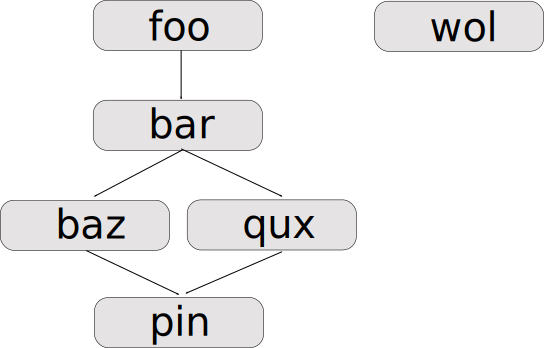
\includegraphics[width=0.4\columnwidth]{resources/tex/cylc-graph}
\end{center}


\subsection{Cycling}

Graph strings allow us to define workflows consisting of tasks. In a suite we
may well want to repeat workflows, which is called cycling.

\begin{center}
    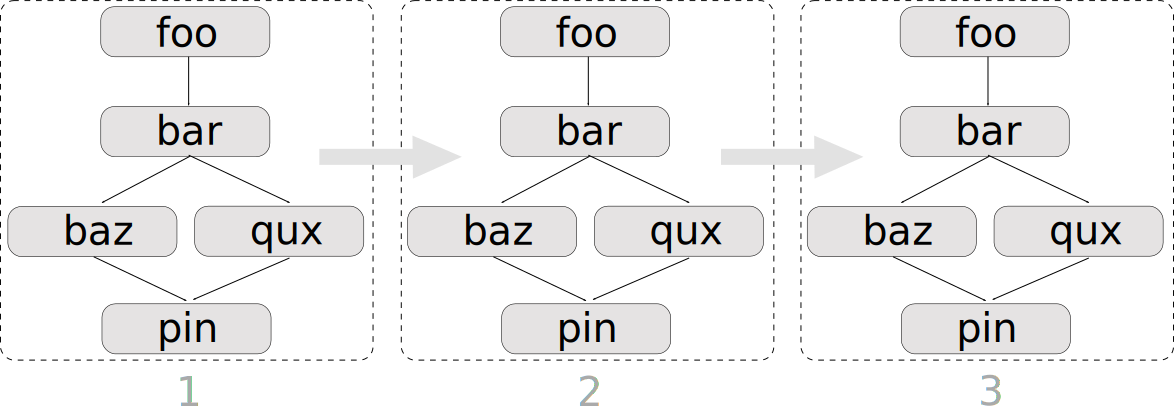
\includegraphics[width=0.6\columnwidth]{resources/tex/cylc-cycle-graph}
\end{center}

The above diagram shows the workflow from the previous example repeated three
times with the resultant cycles numbered 1, 2 and 3. With cylc cycles can
either be numbered or alternatively can use datetimes, for this tutorial shall
use datetimes.

In order to cycle a workflow we need a start point to begin cycling from, and
end point to finish cycling at. In cylc these are defined using the
\lstinline=initial cycle point= and \lstinline=final cycle point= values which
are set in the \lstinline=[scheduling]= section.

We tell cylc to cycle over a workflow using graph section headings. A graph
section heading is a section that sits inside the
\lstinline=[[dependencies]]= section. In the following example the task
\lstinline{foo} will run once every day at midday starting on the 1st of
January 2000 and ending on the 5th of January 2000.

\begin{lstlisting}[language=suiterc]
[scheduling]
    initial cycle point = 2000-01-01T00
    final cycle point = 2000-01-05T00
    [[dependencies]]
        [[[T12]]]
            graph = foo
\end{lstlisting}

In this example the graph section heading \lstinline=[[[T12]]]= means run
the workflow defined in the \lstinline=graph= section once every day at
12:00. Equally \lstinline=[[[T06]]]= means run every day at 06:00 and
\lstinline=[[[T2145]]]= means run every day at 21:45.

\note{When we talk of tasks running every day we don't mean that
the suite waits an entire day before running the next task, cycle points are
just labels we can use to organise cycles. It is possible to set real-world
datetimes as dependencies for cylc tasks see section
\ref{clock-triggered-tasks}.}

There are multiple forms of graph section heading to serve different purposes,
more exotic forms are outlined in section \ref{advanced-cycling}.


\subsection{Inter Cycle Dependence}

In the previous example the task \lstinline{foo} ran once every day. Because
we have not specified any dependencies multiple \lstinline{foo} tasks can end
up running in parallel. In order to make these tasks run one after the other
we will have to specify a dependency across cycle points as in the following
example:

\begin{lstlisting}[language=suiterc]
[scheduling]
    initial cycle point = 2000-01-01T00
    final cycle point = 2000-01-05T00
    [[dependencies]]
        [[[T12]]]
        graph = foo[-P1D] => foo
\end{lstlisting}

The expression \lstinline{foo[-P1D]} means \lstinline{foo} at a cycle point
one day earlier, hence in this example \lstinline{foo} will only run once
its previous run has succeeded. \lstinline{P1D} is an ISO8601 duration (for
details see \url{http://wikipedia.org/wiki/ISO_8601#Durations}), \lstinline=P=
denotes a duration and the \lstinline=1D= part means one day. The minus implies
that the duration is negative (going backwards in time), other examples of
ISO8601 durations are:

\begin{itemize}
    \item \lstinline{-PT12H} (12 hours ago).
    \item \lstinline{-PT6H30M} (6 hours 30 minutes ago).
    \item \lstinline{P1W} (1 week in the future).
\end{itemize}

\paragraph*{Demo}
This demo is an example of a cycling workflow, to run it create a new
directory and create a blank rose-suite.conf file within it.

Next copy the following code into a suite.rc and a bin/count-down file.

\begin{lstlisting}[language=]
|-- bin/
|   `-- count-down
|-- rose-suite.conf
`-- suite.rc
\end{lstlisting}

\begin{lstlisting}[language=suiterc, title=suite.rc]
[scheduling]
    initial cycle point = 2000-01-01T00
    final cycle point = 2000-01-05T00
    [[dependencies]]
        [[[T00]]]
            graph = """
                blast_off[-P1D] => point_upwards
                point_upwards => load_astronauts
                point_upwards => fill_fuel_tank
                point_upwards => set_coordinates
                fill_fuel_tank => light_fuse
                set_coordinates => count_down
                light_fuse => count_down
                load_astronauts => count_down
                count_down => blast_off
            """
[runtime]
    [[point_upwards]]
        script = sleep 2; echo "spikey end pointing at sky, flamey end \
                    pointing at ground"
    [[load_astronauts]]
        script = sleep 1; echo "loaded astronauts"
    [[fill_fuel_tank]]
        script = sleep 5; echo "tank brimmed"
    [[set_coordinates]]
        script = echo "coordinates set for west wallaby st"
    [[light_fuse]]
        script = echo "stand well back"
    [[count_down]]
        script = count-down
    [[blast_off]]
        script = echo "blast off"
\end{lstlisting}

\begin{lstlisting}[language=bash, title=bin/count-down]
sleep 1; echo 5;
sleep 1; echo 4;
sleep 1; echo 3;
sleep 1; echo 2;
sleep 1; echo 1;
\end{lstlisting}

To run this demo suite, enter the following commands:

\begin{lstlisting}[language=bash]
$ chmod +x bin/count-down  # Make the count-down script executable.
$ rose suite-run
\end{lstlisting}

Again a window should open up showing you the progress of the suite.
Whilst the suite is running try entering graph mode by selecting
\lstinline[language=]{View > 1 - Graph View} from the menubar, this will show
the dependencies between the tasks as they run.
